% APÊNDICES--------------------------------------------------------------------
\renewcommand{\figurename}{Quadro}
\setcounter{figure}{0}
\begin{apendicesenv}
\partapendices

% Primeiro apêndice------------------------------------------------------------
\chapter{Descrição dos casos de uso do Sistema Admink}
\label{chap:apendiceA}

    \begin{figure}[!htb]
	    \centering
	    \sbox0{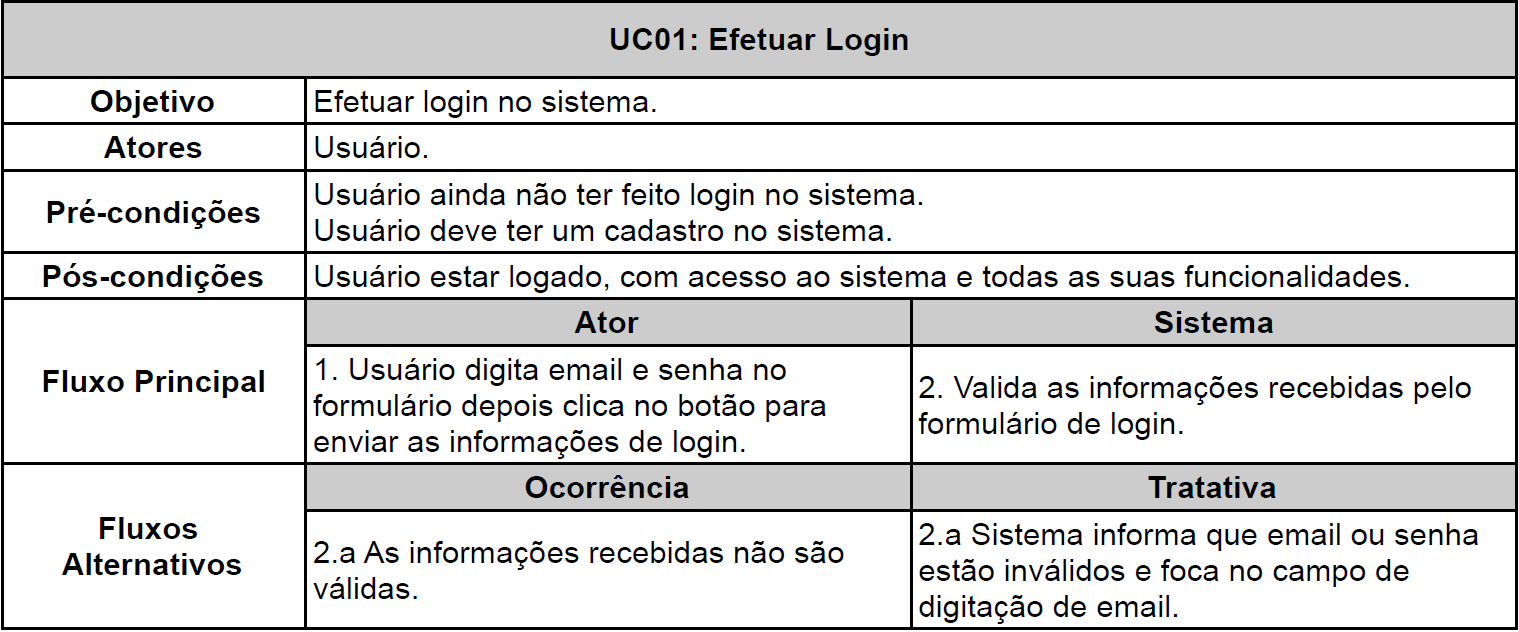
\includegraphics[width=1\textwidth]{./assets/apendices/UC01Admink}}% measure width
	    \begin{minipage}{\wd0}
		    \usebox0
		    \caption[]{UC01: Efetuar Login}
		    \label{fig:uc1-admink}
		    \fonte{o Autor}
	    \end{minipage}
    \end{figure}
    

    \begin{figure}[!htb]
	    \centering
	    \sbox0{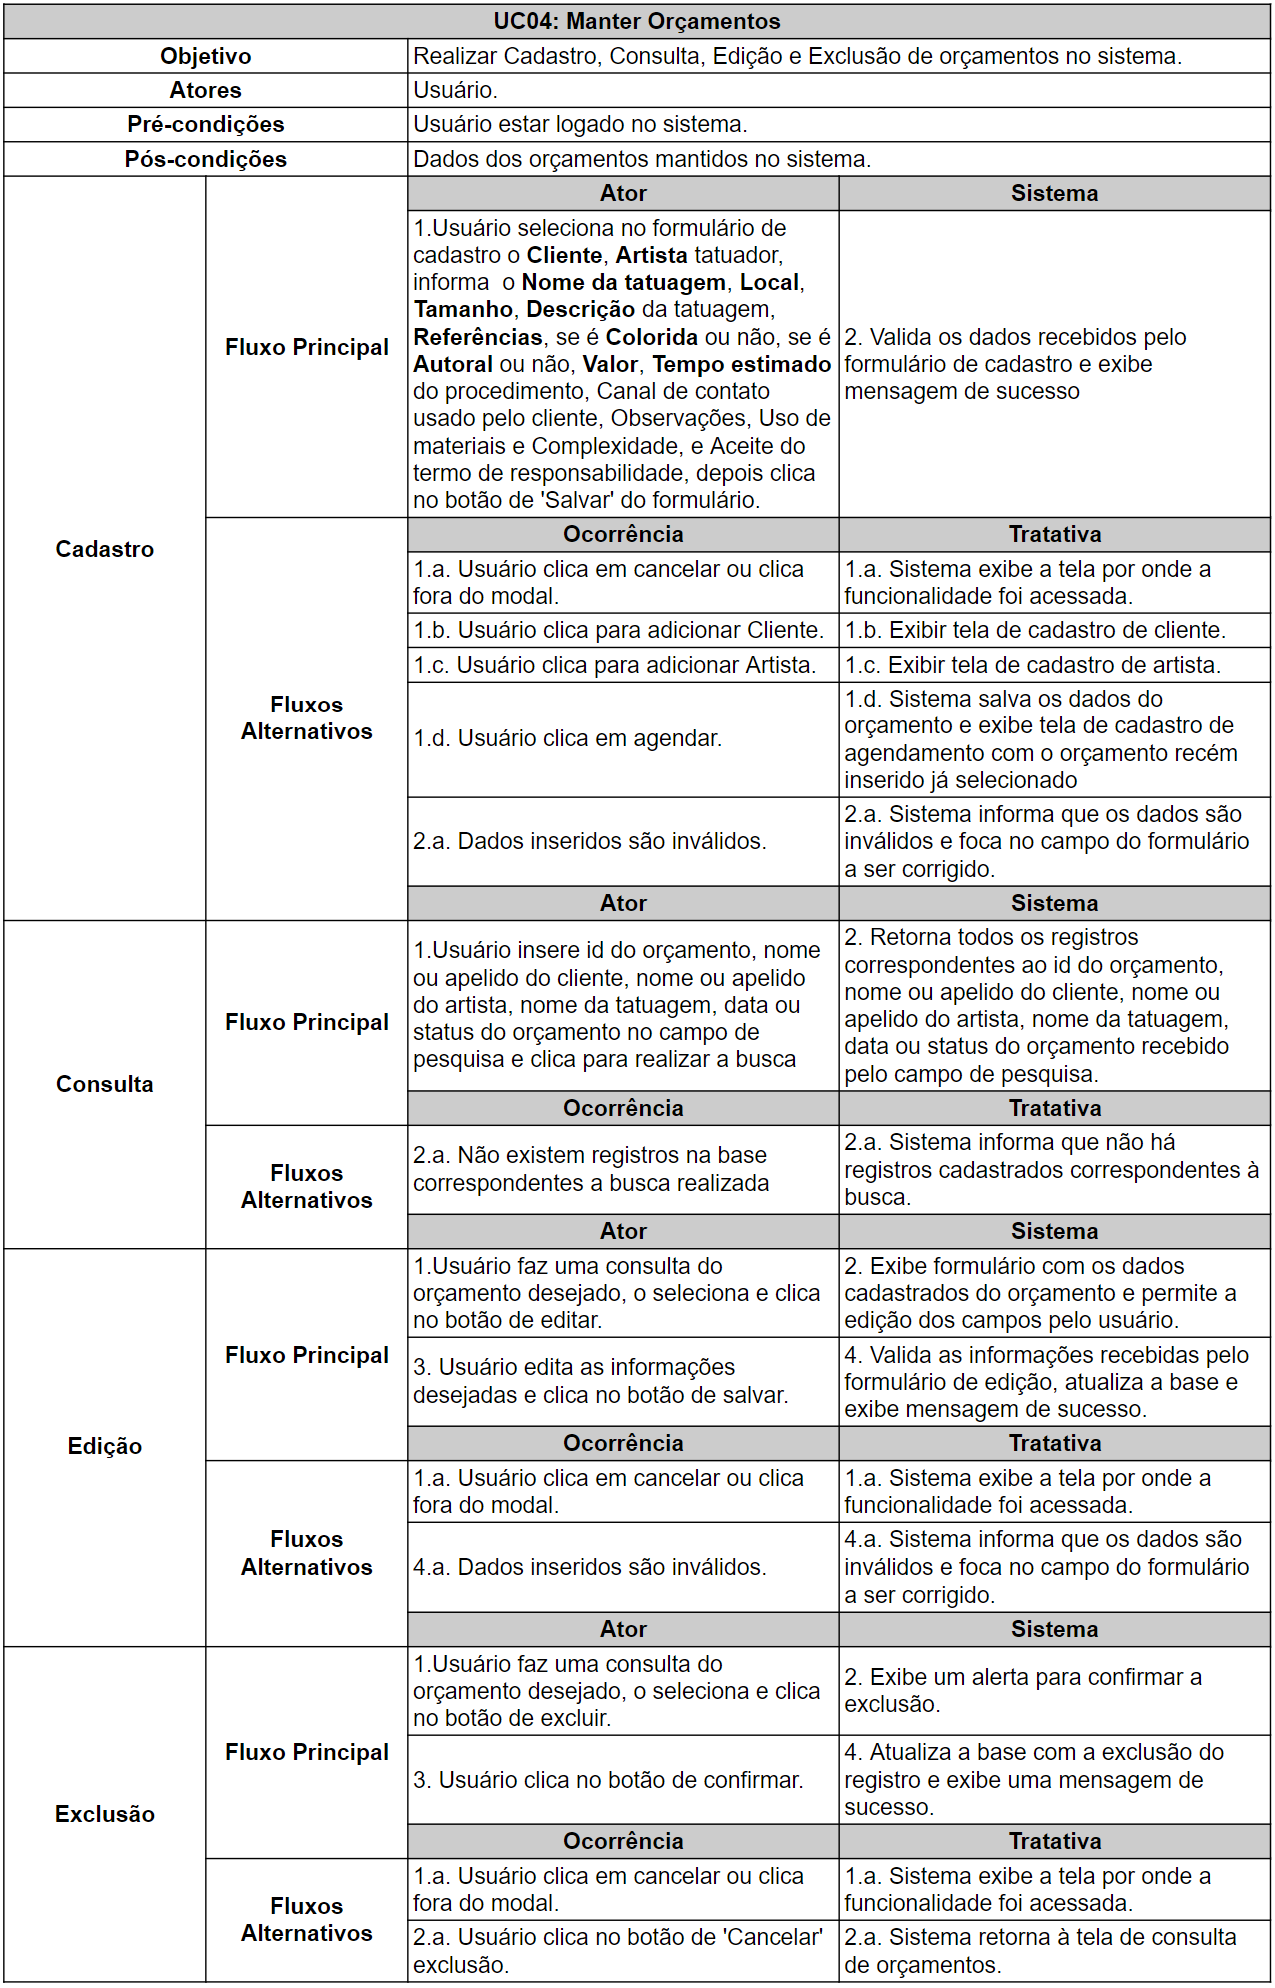
\includegraphics[width=1\textwidth]{./assets/apendices/UC04Admink}}% measure width
	    \begin{minipage}{\wd0}
		    \usebox0
		    \caption[]{UC04: Manter Orçamentos}
		    \label{fig:uc4-admink}
		    \fonte{o Autor}
	    \end{minipage}
    \end{figure}

\chapter{Plano de Testes do Sistema Admink}
\label{chap:apendiceB}

\setcounter{figure}{0}

    \begin{figure}[!htb]
	    \centering
	    \sbox0{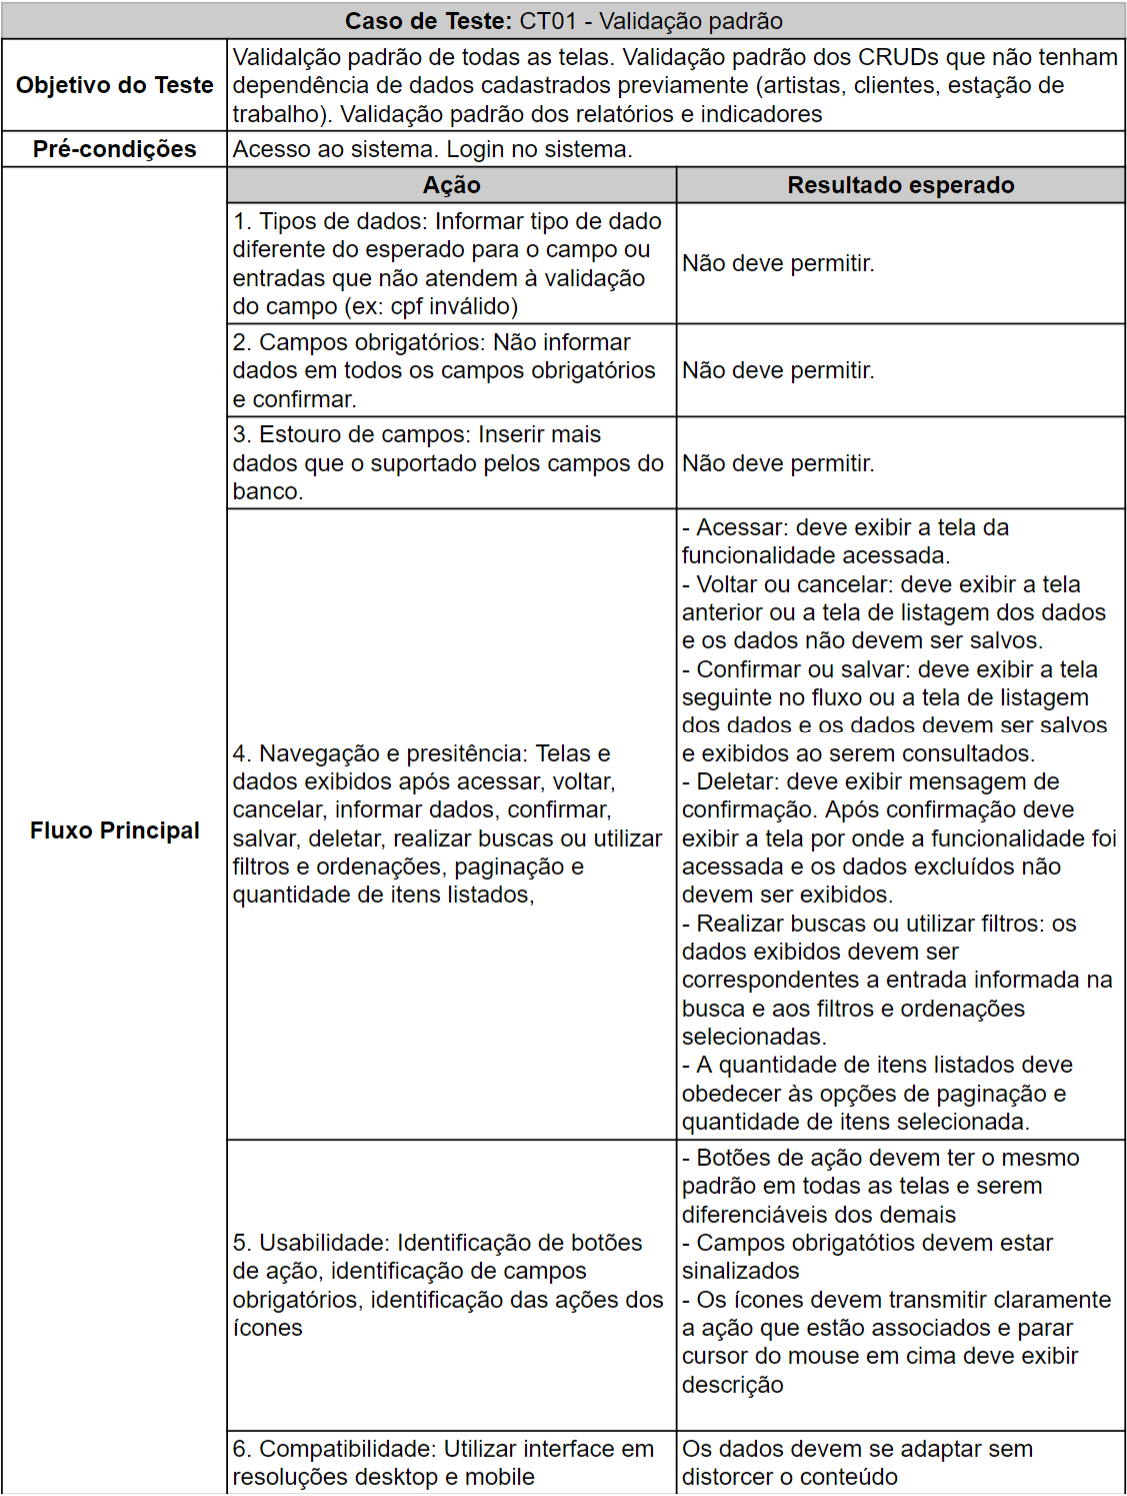
\includegraphics[width=1\textwidth]{./assets/apendices/CT01Admink}}% measure width
	    \begin{minipage}{\wd0}
		    \usebox0
		    \caption[]{TC01: Validação Padrão}
		    \label{fig:tc01-admink}
		    \fonte{o Autor}
	    \end{minipage}
    \end{figure}
    
    \begin{figure}[!htb]
	    \centering
	    \sbox0{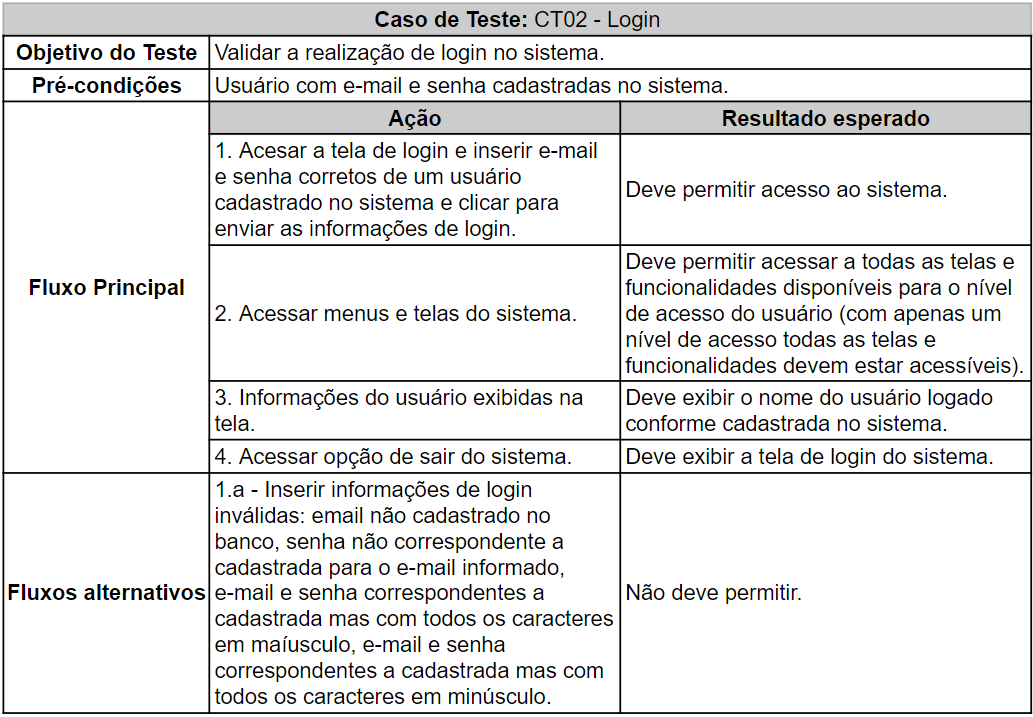
\includegraphics[width=1\textwidth]{./assets/apendices/CT02Admink}}% measure width
	    \begin{minipage}{\wd0}
		    \usebox0
		    \caption[]{TC02: Login}
		    \label{fig:tc02-admink}
		    \fonte{o Autor}
	    \end{minipage}
    \end{figure}
    
    \begin{figure}[!htb]
	    \centering
	    \sbox0{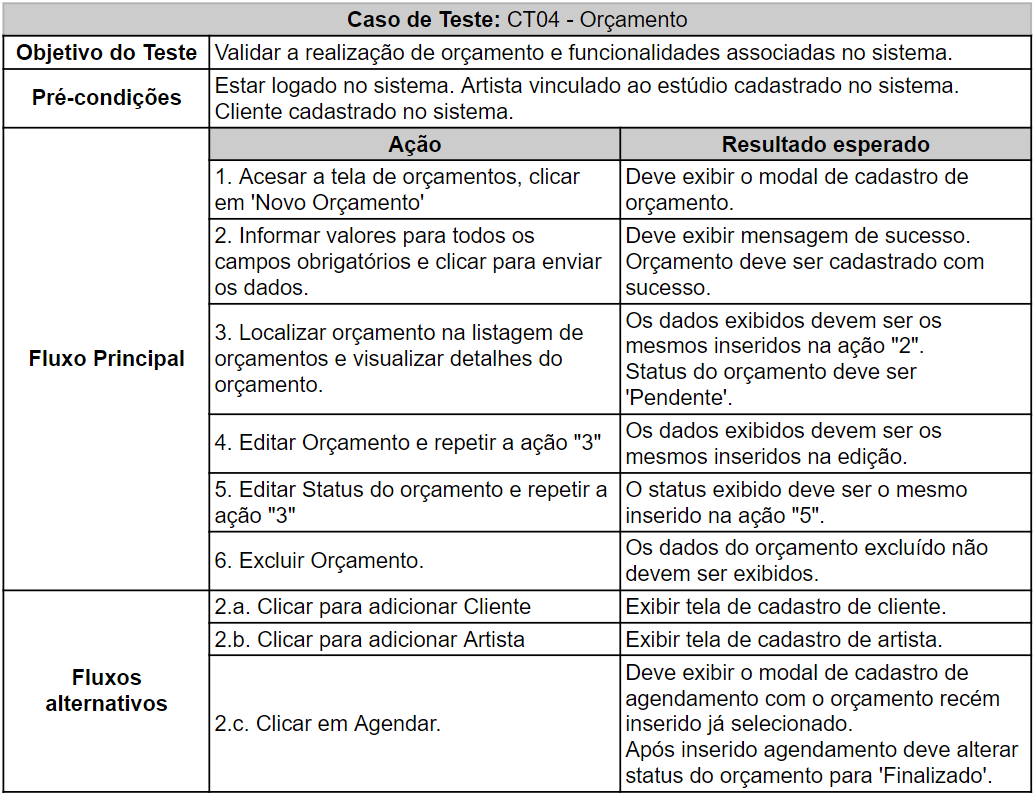
\includegraphics[width=1\textwidth]{./assets/apendices/CT04Admink}}% measure width
	    \begin{minipage}{\wd0}
		    \usebox0
		    \caption[]{TC04: Orçamento}
		    \label{fig:tc04-admink}
		    \fonte{o Autor}
	    \end{minipage}
    \end{figure}
    
\chapter{Scripts de Teste de Integração do Sistema Admink}
\label{chap:apendiceC}

\begin{lstlisting}[language=PHP, caption= Scripts de teste de Login, nolol,
label={code:LoginTest}]

<?php

namespace Tests\Integration\Login;

use Tests\TestCase;
use App\User;

class LoginTest extends TestCase
{

    public function teste1LoginComSucessoComEmailESenhaValidos()
    {
        $user = factory(User::class)->create();
        $response = $this->call('POST', '/login', ['email' => $user->email, 'password' => 'teste@123']);
        $response->assertStatus(302);
        $response->assertRedirect('/admin/home');
    }

    public function teste2LogincomFalhaComEmailInvalido()
    {
        $user = factory(User::class)->create();
        $response = $this->call('POST', '/login', ['email' => 'invalido@email.com', 'password' => 'teste@123']);
        $response->assertStatus(302);
        $response->assertRedirect('/');
    }

    public function teste3LogincomFalhaComEmailESenhaVazios()
    {
        $user = factory(User::class)->create();
        $response = $this->call('POST', '/login', ['email' => '', 'password' => '']);
        $response->assertStatus(302);
        $response->assertRedirect('/');
    }
    public function teste4LogincomFalhaComEmailESenhaNulos()
    {
        $user = factory(User::class)->create();
        $response = $this->call('POST', '/login', ['email' => null, 'password' => null]);
        $response->assertStatus(302);
        $response->assertRedirect('/');
    }

    public function teste5LogincomFalhaComSenhaIncorreta()
    {
        $user = factory(User::class)->create();
        $response = $this->call('POST', '/login', ['email' => $user->email, 'password' => 'wrongpassowrd']);
        $response->assertStatus(302);
        $response->assertRedirect('/');
    }
}
    
\end{lstlisting}

\fonte{o Autor}

\begin{lstlisting}[language=PHP, caption= Scripts de teste de Criação de Orçamentos, nolol,
label={code:CriacaoDeOrcamentoTest}]
<?php

namespace Tests\Integration\Orcamentos;

use Tests\TestCase;
use App\User;
use App\EstudioUsers;
use App\Estudio;
use App\Cliente;
use App\Artista;
use App\ArtistaEstudio;
use App\ClienteEstudio;


class CriacaoDeOrcamentoTest extends TestCase
{
    public function teste1CriacaoDeOrcamentoComSucessoDadosCorretos()
    {
        $user = factory(User::class)->create();
        $estudio = factory(Estudio::class)->create();
        factory(EstudioUsers::class)->create(['fk_users_id_users' => $user->id, 'fk_estudio_id_estudio' => $estudio->id_estudio]);
        $artista = factory(Artista::class)->create();
        $cliente = factory(Cliente::class)->create();
        factory(ArtistaEstudio::class)->create(['fk_artista_id_artista' => $artista->id_artista, 'fk_estudio_id_estudio' => $estudio->id_estudio]);
        factory(ClienteEstudio::class)->create(['fk_cliente_id_cliente' => $cliente->id_cliente, 'fk_estudio_id_estudio' => $estudio->id_estudio]);


        $response = $this->actingAs($user)
            ->post('/admin/orcamentos', [
                'cliente'               => $cliente->id_cliente,
                'artista'               => $artista->id_artista,
                'tatuagem_nome'         => 'Teste Orçamento',
                'tatuagem_local'        => 'Teste',
                'tatuagem_comprimento'  => 10,
                'tatuagem_largura'      => 10,
                'tatuagem_descricao'    => 'Teste Orçamento Criado com Sucesso!',
                'tatuagem_referencias'  => null,
                'canal_contato'         => null,
                'tempo_estimado'        => null,
                'valor'                 => null,
                'uso_materiais'         => null,
                'complexidade'          => null,
                'observacao'            => null
            ]);
        $response->assertStatus(302);
        $response->assertSessionHas('success_toastr', 'O orçamento foi cadastrado com sucesso!');
    }

    public function teste2CriacaoDeOrcamentoComFalhaDadosObrigatorioVazios()
    {
        $user = factory(User::class)->create();
        $estudio = factory(Estudio::class)->create();
        factory(EstudioUsers::class)->create(['fk_users_id_users' => $user->id, 'fk_estudio_id_estudio' => $estudio->id_estudio]);

        $response = $this->actingAs($user)
            ->post('/admin/orcamentos', [
                'cliente'               => null,
                'artista'               => null,
                'tatuagem_nome'         => '',
                'tatuagem_local'        => '',
                'tatuagem_comprimento'  => null,
                'tatuagem_largura'      => null,
                'tatuagem_descricao'    => '',
                'tatuagem_referencias'  => null,
                'canal_contato'         => null,
                'tempo_estimado'        => null,
                'valor'                 => null,
                'uso_materiais'         => null,
                'complexidade'          => null,
                'observacao'            => null
            ]);

        $response->assertStatus(302);
        $this->assertEquals(session('errors')->get('cliente')[0], 'O campo cliente é obrigatório.');
        $this->assertEquals(session('errors')->get('artista')[0], 'O campo artista é obrigatório.');
        $this->assertEquals(session('errors')->get('tatuagem_nome')[0], 'O campo tatuagem nome é obrigatório.');
        $this->assertEquals(session('errors')->get('tatuagem_local')[0], 'O campo tatuagem local é obrigatório.');
        $this->assertEquals(session('errors')->get('tatuagem_comprimento')[0], 'O campo tatuagem comprimento é obrigatório.');
        $this->assertEquals(session('errors')->get('tatuagem_largura')[0], 'O campo tatuagem largura é obrigatório.');
        $this->assertEquals(session('errors')->get('tatuagem_descricao')[0], 'O campo tatuagem descricao é obrigatório.');
    }

    public function teste3CriacaoDeOrcamentoComFalhaDadosComTamanhoMaiorQueOSuportado()
    {
        include  'TestStrings.php';
        $user = factory(User::class)->create();
        $estudio = factory(Estudio::class)->create();
        factory(EstudioUsers::class)->create(['fk_users_id_users' => $user->id, 'fk_estudio_id_estudio' => $estudio->id_estudio]);

        $response = $this->actingAs($user)
            ->post('/admin/orcamentos', [
                'cliente'               => 2147483648,
                'artista'               => 2147483648,
                'tatuagem_nome'         => 'String com 61 caracteres  TETESTETESTETESTETESTETESTETESTETES',
                'tatuagem_local'        => 'String com 61 caracteres  TETESTETESTETESTETESTETESTETESTETES',
                'tatuagem_comprimento'  => 201,
                'tatuagem_largura'      => 201,
                'tatuagem_descricao'    => 'String com 256 caracteres ESTETESTETESTETESTETESTETESTETESTETESTETESTETESTETESTETESTETESTETESTETESTETESTETESTETESTETESTETESTETESTETESTETESTETESTETESTETESTETESTETESTETESTETESTETESTETESTETESTETESTETESTETESTETESTETESTETESTETESTETESTETESTETESTETESTETESTETESTET',
                'tatuagem_referencias'  => $stringCom65536caracteres,
                'canal_contato'         => 2147483648,
                'tempo_estimado'        => '24:00:00',
                'valor'                 => 100000,
                'uso_materiais'         => 2147483648,
                'complexidade'          => 2147483648,
                'observacao'            => 'String com 256 caracteres ESTETESTETESTETESTETESTETESTETESTETESTETESTETESTETESTETESTETESTETESTETESTETESTETESTETESTETESTETESTETESTETESTETESTETESTETESTETESTETESTETESTETESTETESTETESTETESTETESTETESTETESTETESTETESTETESTETESTETESTETESTETESTETESTETESTETESTETESTET'
            ]);

        $response->assertStatus(302);
        $this->assertEquals(session('errors')->get('tatuagem_nome')[0], 'O campo tatuagem nome não pode ser superior a 60 caracteres.');
        $this->assertEquals(session('errors')->get('tatuagem_local')[0], 'O campo tatuagem local não pode ser superior a 60 caracteres.');
        $this->assertEquals(session('errors')->get('tatuagem_comprimento')[0], 'O campo tatuagem comprimento não pode ser superior a 200.');
        $this->assertEquals(session('errors')->get('tatuagem_largura')[0], 'O campo tatuagem largura não pode ser superior a 200.');
        $this->assertEquals(session('errors')->get('tatuagem_descricao')[0], 'O campo tatuagem descricao não pode ser superior a 255 caracteres.');
        $this->assertEquals(session('errors')->get('valor')[0], 'O valor do orçamento deve estar entre R$ 0,00 e R$ 99.999,99');
        $this->assertEquals(session('errors')->get('tempo_estimado')[0], 'O tempo estimado deve estar entre 00:00 e 23:59');
        $this->assertEquals(session('errors')->get('observacao')[0], 'O campo observacao não pode ser superior a 255 caracteres.');
    }

    public function teste4CriacaoDeOrcamentoComFalhaDadosComTiposDiferentesDoSuportado()
    {
        $user = factory(User::class)->create();
        $estudio = factory(Estudio::class)->create();
        factory(EstudioUsers::class)->create(['fk_users_id_users' => $user->id, 'fk_estudio_id_estudio' => $estudio->id_estudio]);

        $response = $this->actingAs($user)
            ->post('/admin/orcamentos', [
                'cliente'               => 'String ao invés de inteiro',
                'artista'               => 'String ao invés de inteiro',
                'tatuagem_nome'         => 73273,
                'tatuagem_local'        => 73273,
                'tatuagem_comprimento'  => 'String ao invés de inteiro',
                'tatuagem_largura'      => 'String ao invés de inteiro',
                'tatuagem_descricao'    => ['array ao invés', 'de string'],
                'tatuagem_referencias'  => 73273,
                'canal_contato'         => ['array ao invés', 'de string'],
                'tempo_estimado'        => 1643067873,
                'valor'                 => 'String ao invés de float',
                'uso_materiais'         => 'String ao invés de inteiro',
                'complexidade'          => 'String ao invés de inteiro',
                'observacao'            => 'String com 256 caracteres ESTETESTETESTETESTETESTETESTETESTETESTETESTETESTETESTETESTETESTETESTETESTETESTETESTETESTETESTETESTETESTETESTETESTETESTETESTETESTETESTETESTETESTETESTETESTETESTETESTETESTETESTETESTETESTETESTETESTETESTETESTETESTETESTETESTETESTETESTET'
            ]);

        $response->assertStatus(302);
        $this->assertEquals(session('errors')->get('tatuagem_nome')[0], 'O campo tatuagem nome deve ser uma string.');
        $this->assertEquals(session('errors')->get('tatuagem_local')[0], 'O campo tatuagem local deve ser uma string.');
        $this->assertEquals(session('errors')->get('tatuagem_comprimento')[0], 'O campo tatuagem comprimento deve ser um número.');
        $this->assertEquals(session('errors')->get('tatuagem_largura')[0], 'O campo tatuagem largura deve ser um número.');
        $this->assertEquals(session('errors')->get('tatuagem_descricao')[0], 'O campo tatuagem descricao deve ser uma string.');
        $this->assertEquals(session('errors')->get('valor')[0], 'O valor do orçamento deve estar entre R$ 0,00 e R$ 99.999,99');
        $this->assertEquals(session('errors')->get('tempo_estimado')[0], 'O tempo estimado deve estar entre 00:00 e 23:59');
        $this->assertEquals(session('errors')->get('observacao')[0], 'O campo observacao não pode ser superior a 255 caracteres.');
    }
}
    
\end{lstlisting}

\fonte{o Autor}

\begin{lstlisting}[language=PHP, caption= Scripts de teste de Edição de Orçamentos, nolol,
label={code:EdicaoDeOrcamentoTest}]
<?php

namespace Tests\Integration\Orcamentos;

use Tests\TestCase;
use App\User;
use App\EstudioUsers;
use App\Orcamento;
use App\Estudio;
use App\Cliente;
use App\Artista;
use App\ArtistaEstudio;
use App\ClienteEstudio;

class EdicaoDeOrcamentosTest extends TestCase
{

    public function teste1EdicaoDeOrcamentoComSucessoSemDadosDeTatuador()
    {
        $user = factory(User::class)->create();
        $estudio = factory(Estudio::class)->create();
        factory(EstudioUsers::class)->create(['fk_users_id_users' => $user->id, 'fk_estudio_id_estudio' => $estudio->id_estudio]);
        $artista = factory(Artista::class)->create();
        $cliente = factory(Cliente::class)->create();
        factory(ArtistaEstudio::class)->create(['fk_artista_id_artista' => $artista->id_artista, 'fk_estudio_id_estudio' => $estudio->id_estudio]);
        factory(ClienteEstudio::class)->create(['fk_cliente_id_cliente' => $cliente->id_cliente, 'fk_estudio_id_estudio' => $estudio->id_estudio]);
        $orcamento = factory(Orcamento::class)->create(['fk_cliente_id_cliente' => $cliente->id_cliente, 'fk_artista_id_artista' => $artista->id_artista, 'fk_estudio_id_estudio' => $estudio->id_estudio, 'fk_orcamento_status_id_orcamento_status' => 1]);

        $response = $this->actingAs($user)
            ->post('/admin/orcamentos/' . $orcamento->id_orcamento, [
                '_method'               => 'PUT',
                'cliente'               => $cliente->id_cliente,
                'artista'               => $artista->id_artista,
                'tatuagem_nome'         => 'Teste Edição Orçamento',
                'tatuagem_local'        => 'Teste Edição Orçamento',
                'tatuagem_comprimento'  => 13,
                'tatuagem_largura'      => 13,
                'tatuagem_descricao'    => 'Teste Orçamento Editado com Sucesso!',
                'tatuagem_referencias'  => 'testeedicaoorcamento.com.br',
                'canal_contato'         => 'Teste Edição',
                'tempo_estimado'        => null,
                'valor'                 => null,
                'uso_materiais'         => null,
                'complexidade'          => null,
                'observacao'            => null
            ]);
        $response->assertStatus(302);
        $response->assertSessionHas('success_toastr', 'O orçamento foi atualizado com sucesso!');
    }

    public function teste2EdicaoDeOrcamentoComSucessoComDadosDeTatuador()
    {
        $user = factory(User::class)->create();
        $estudio = factory(Estudio::class)->create();
        factory(EstudioUsers::class)->create(['fk_users_id_users' => $user->id, 'fk_estudio_id_estudio' => $estudio->id_estudio]);
        $artista = factory(Artista::class)->create();
        $cliente = factory(Cliente::class)->create();
        factory(ArtistaEstudio::class)->create(['fk_artista_id_artista' => $artista->id_artista, 'fk_estudio_id_estudio' => $estudio->id_estudio]);
        factory(ClienteEstudio::class)->create(['fk_cliente_id_cliente' => $cliente->id_cliente, 'fk_estudio_id_estudio' => $estudio->id_estudio]);
        $orcamento = factory(Orcamento::class)->create(['fk_cliente_id_cliente' => $cliente->id_cliente, 'fk_artista_id_artista' => $artista->id_artista, 'fk_estudio_id_estudio' => $estudio->id_estudio, 'fk_orcamento_status_id_orcamento_status' => 1]);

        $response = $this->actingAs($user)
            ->post('/admin/orcamentos/' . $orcamento->id_orcamento, [
                '_method'               => 'PUT',
                'cliente'               => $cliente->id_cliente,
                'artista'               => $artista->id_artista,
                'tatuagem_nome'         => 'Teste Edição Orçamento',
                'tatuagem_local'        => 'Teste Edição Orçamento',
                'tatuagem_comprimento'  => 13,
                'tatuagem_largura'      => 13,
                'tatuagem_descricao'    => 'Teste Orçamento Editado com Sucesso!',
                'tatuagem_referencias'  => 'testeedicaoorcamento.com.br',
                'canal_contato'         => 'Teste Edição',
                'tempo_estimado'        => '03:00',
                'valor'                 => '13,00',
                'uso_materiais'         => 1,
                'complexidade'          => 1,
                'observacao'            => 'Teste Edição de Orçamento com sucesso com dados de tatuador!'
            ]);
        $response->assertStatus(302);
        $response->assertSessionHas('success_toastr', 'O orçamento foi atualizado com sucesso!');
    }

    public function teste3EdicaoDeOrcamentoComFalhaDadosObrigatoriosVazios()
    {
        $user = factory(User::class)->create();
        $estudio = factory(Estudio::class)->create();
        factory(EstudioUsers::class)->create(['fk_users_id_users' => $user->id, 'fk_estudio_id_estudio' => $estudio->id_estudio]);
        $artista = factory(Artista::class)->create();
        $cliente = factory(Cliente::class)->create();
        factory(ArtistaEstudio::class)->create(['fk_artista_id_artista' => $artista->id_artista, 'fk_estudio_id_estudio' => $estudio->id_estudio]);
        factory(ClienteEstudio::class)->create(['fk_cliente_id_cliente' => $cliente->id_cliente, 'fk_estudio_id_estudio' => $estudio->id_estudio]);
        $orcamento = factory(Orcamento::class)->create(['fk_cliente_id_cliente' => $cliente->id_cliente, 'fk_artista_id_artista' => $artista->id_artista, 'fk_estudio_id_estudio' => $estudio->id_estudio, 'fk_orcamento_status_id_orcamento_status' => 1]);

        $response = $this->actingAs($user)
            ->post('/admin/orcamentos/' . $orcamento->id_orcamento, [
                '_method'               => 'PUT',
                'cliente'               => null,
                'artista'               => null,
                'tatuagem_nome'         => '',
                'tatuagem_local'        => '',
                'tatuagem_comprimento'  => null,
                'tatuagem_largura'      => null,
                'tatuagem_descricao'    => '',
                'tatuagem_referencias'  => null,
                'canal_contato'         => null,
                'tempo_estimado'        => null,
                'valor'                 => null,
                'uso_materiais'         => null,
                'complexidade'          => null,
                'observacao'            => null
            ]);
        $response->assertStatus(302);
        $this->assertEquals(session('errors')->get('cliente')[0], 'O campo cliente é obrigatório.');
        $this->assertEquals(session('errors')->get('artista')[0], 'O campo artista é obrigatório.');
        $this->assertEquals(session('errors')->get('tatuagem_nome')[0], 'O campo tatuagem nome é obrigatório.');
        $this->assertEquals(session('errors')->get('tatuagem_local')[0], 'O campo tatuagem local é obrigatório.');
        $this->assertEquals(session('errors')->get('tatuagem_comprimento')[0], 'O campo tatuagem comprimento é obrigatório.');
        $this->assertEquals(session('errors')->get('tatuagem_largura')[0], 'O campo tatuagem largura é obrigatório.');
        $this->assertEquals(session('errors')->get('tatuagem_descricao')[0], 'O campo tatuagem descricao é obrigatório.');
    }

    public function teste4EdicaoDeOrcamentoComFalhaDadosComTamanhoMaiorQueOSuportado()
    {   
        include  'TestStrings.php';
        $user = factory(User::class)->create();
        $estudio = factory(Estudio::class)->create();
        factory(EstudioUsers::class)->create(['fk_users_id_users' => $user->id, 'fk_estudio_id_estudio' => $estudio->id_estudio]);
        $artista = factory(Artista::class)->create();
        $cliente = factory(Cliente::class)->create();
        factory(ArtistaEstudio::class)->create(['fk_artista_id_artista' => $artista->id_artista, 'fk_estudio_id_estudio' => $estudio->id_estudio]);
        factory(ClienteEstudio::class)->create(['fk_cliente_id_cliente' => $cliente->id_cliente, 'fk_estudio_id_estudio' => $estudio->id_estudio]);
        $orcamento = factory(Orcamento::class)->create(['fk_cliente_id_cliente' => $cliente->id_cliente, 'fk_artista_id_artista' => $artista->id_artista, 'fk_estudio_id_estudio' => $estudio->id_estudio, 'fk_orcamento_status_id_orcamento_status' => 1]);
        
        $response = $this->actingAs($user)
            ->post('/admin/orcamentos/' . $orcamento->id_orcamento, [
                '_method'               => 'PUT',
                'cliente'               => 2147483648,
                'artista'               => 2147483648,
                'tatuagem_nome'         => $stringCom61Caracteres,
                'tatuagem_local'        => $stringCom61Caracteres,
                'tatuagem_comprimento'  => 201,
                'tatuagem_largura'      => 201,
                'tatuagem_descricao'    => $stringCom256Caracteres,
                'tatuagem_referencias'  => $stringCom65536Caracteres,
                'canal_contato'         => 2147483648,
                'tempo_estimado'        => '24:00:00',
                'valor'                 => '100.000,00',
                'uso_materiais'         => 2147483648,
                'complexidade'          => 2147483648,
                'observacao'            => $stringCom256Caracteres
            ]);

        $response->assertStatus(302);
        $this->assertEquals(session('errors')->get('tatuagem_nome')[0], 'O campo tatuagem nome não pode ser superior a 60 caracteres.');
        $this->assertEquals(session('errors')->get('tatuagem_local')[0], 'O campo tatuagem local não pode ser superior a 60 caracteres.');
        $this->assertEquals(session('errors')->get('tatuagem_comprimento')[0], 'O campo tatuagem comprimento não pode ser superior a 200.');
        $this->assertEquals(session('errors')->get('tatuagem_largura')[0], 'O campo tatuagem largura não pode ser superior a 200.');
        $this->assertEquals(session('errors')->get('tatuagem_descricao')[0], 'O campo tatuagem descricao não pode ser superior a 255 caracteres.');
        $this->assertEquals(session('errors')->get('valor')[0], 'O campo valor tem um formato inválido.');
        $this->assertEquals(session('errors')->get('tempo_estimado')[0], 'O campo tempo estimado tem um formato inválido.');
        $this->assertEquals(session('errors')->get('observacao')[0], 'O campo observacao não pode ser superior a 255 caracteres.');
    }

    public function teste5EdicaoDeOrcamentoComFalhaDadosComTiposDiferentesDoSuportado()
    {
        include  'TestStrings.php';
        $user = factory(User::class)->create();
        $estudio = factory(Estudio::class)->create();
        factory(EstudioUsers::class)->create(['fk_users_id_users' => $user->id, 'fk_estudio_id_estudio' => $estudio->id_estudio]);
        $artista = factory(Artista::class)->create();
        $cliente = factory(Cliente::class)->create();
        factory(ArtistaEstudio::class)->create(['fk_artista_id_artista' => $artista->id_artista, 'fk_estudio_id_estudio' => $estudio->id_estudio]);
        factory(ClienteEstudio::class)->create(['fk_cliente_id_cliente' => $cliente->id_cliente, 'fk_estudio_id_estudio' => $estudio->id_estudio]);
        $orcamento = factory(Orcamento::class)->create(['fk_cliente_id_cliente' => $cliente->id_cliente, 'fk_artista_id_artista' => $artista->id_artista, 'fk_estudio_id_estudio' => $estudio->id_estudio, 'fk_orcamento_status_id_orcamento_status' => 1]);

        $response = $this->actingAs($user)
            ->post('/admin/orcamentos/' . $orcamento->id_orcamento, [
                '_method'               => 'PUT',
                'cliente'               => 'String ao invés de inteiro',
                'artista'               => 'String ao invés de inteiro',
                'tatuagem_nome'         => 73273,
                'tatuagem_local'        => 73273,
                'tatuagem_comprimento'  => 'String ao invés de inteiro',
                'tatuagem_largura'      => 'String ao invés de inteiro',
                'tatuagem_descricao'    => ['array ao invés', 'de string'],
                'tatuagem_referencias'  => 73273,
                'canal_contato'         => ['array ao invés', 'de string'],
                'tempo_estimado'        => 1643067873,
                'valor'                 => 100000.00,
                'uso_materiais'         => 'String ao invés de inteiro',
                'complexidade'          => 'String ao invés de inteiro',
                'observacao'            => $stringCom256Caracteres
            ]);
        $response->assertStatus(302);
        $this->assertEquals(session('errors')->get('tatuagem_nome')[0], 'O campo tatuagem nome deve ser uma string.');
        $this->assertEquals(session('errors')->get('tatuagem_local')[0], 'O campo tatuagem local deve ser uma string.');
        $this->assertEquals(session('errors')->get('tatuagem_comprimento')[0], 'O campo tatuagem comprimento deve ser um número.');
        $this->assertEquals(session('errors')->get('tatuagem_largura')[0], 'O campo tatuagem largura deve ser um número.');
        $this->assertEquals(session('errors')->get('tatuagem_descricao')[0], 'O campo tatuagem descricao deve ser uma string.');
        $this->assertEquals(session('errors')->get('valor')[0], 'O campo valor tem um formato inválido.');
        $this->assertEquals(session('errors')->get('tempo_estimado')[0], 'O campo tempo estimado tem um formato inválido.');
        $this->assertEquals(session('errors')->get('observacao')[0], 'O campo observacao não pode ser superior a 255 caracteres.');
    }
}
\end{lstlisting}

\fonte{o Autor}

\begin{lstlisting}[language=PHP, caption= Scripts de teste de Listagem e Deleção de Orçamentos, nolol,
label={code:ListagemEDelecaoDeOrcamentosTest}]
<?php

namespace Tests\Integration\Orcamentos;

use Tests\TestCase;
use App\User;
use App\EstudioUsers;
use App\Orcamento;
use App\Estudio;
use App\Cliente;
use App\Artista;
use App\ArtistaEstudio;
use App\ClienteEstudio;
use App\Estacao;
use App\Agendamento;

class ListagemEDelecaoDeOrcamentosTest extends TestCase
{

    public function teste1ListagemDeOrcamentosComSucesso()
    {
        $user = factory(User::class)->create();
        $estudio = factory(Estudio::class)->create();
        factory(EstudioUsers::class)->create(['fk_users_id_users' => $user->id, 'fk_estudio_id_estudio' => $estudio->id_estudio]);
        $artista = factory(Artista::class)->create();
        $cliente = factory(Cliente::class)->create();
        factory(ArtistaEstudio::class)->create(['fk_artista_id_artista' => $artista->id_artista, 'fk_estudio_id_estudio' => $estudio->id_estudio]);
        factory(ClienteEstudio::class)->create(['fk_cliente_id_cliente' => $cliente->id_cliente, 'fk_estudio_id_estudio' => $estudio->id_estudio]);
        $orcamento = factory(Orcamento::class)->create(['fk_cliente_id_cliente' => $cliente->id_cliente, 'fk_artista_id_artista' => $artista->id_artista, 'fk_estudio_id_estudio' => $estudio->id_estudio, 'fk_orcamento_status_id_orcamento_status' => 1]);
        $orcamento2 = factory(Orcamento::class)->create(['fk_cliente_id_cliente' => $cliente->id_cliente, 'fk_artista_id_artista' => $artista->id_artista, 'fk_estudio_id_estudio' => $estudio->id_estudio, 'fk_orcamento_status_id_orcamento_status' => 1]);

        $response = $this->actingAs($user)
            ->get('/admin/orcamentos');

        $response->assertStatus(200);
        $response->assertSee('<td class="align-middle">' . $orcamento->tatuagem_nome . '</td>', $escaped = false);
        $response->assertSee('<td class="align-middle">#' . str_pad($orcamento->id_orcamento, 5, '0', STR_PAD_LEFT) . '</td>', $escaped = false);
        $response->assertSee('<td class="align-middle">' . $orcamento2->tatuagem_nome . '</td>', $escaped = false);
        $response->assertSee('<td class="align-middle">#' . str_pad($orcamento2->id_orcamento, 5, '0', STR_PAD_LEFT) . '</td>', $escaped = false);
    }

    public function teste2ExclusaoDeOrcamentoNaoAgendadoComSucesso()
    {
        $user = factory(User::class)->create();
        $estudio = factory(Estudio::class)->create();
        factory(EstudioUsers::class)->create(['fk_users_id_users' => $user->id, 'fk_estudio_id_estudio' => $estudio->id_estudio]);
        $artista = factory(Artista::class)->create();
        $cliente = factory(Cliente::class)->create();
        factory(ArtistaEstudio::class)->create(['fk_artista_id_artista' => $artista->id_artista, 'fk_estudio_id_estudio' => $estudio->id_estudio]);
        factory(ClienteEstudio::class)->create(['fk_cliente_id_cliente' => $cliente->id_cliente, 'fk_estudio_id_estudio' => $estudio->id_estudio]);
        $orcamento = factory(Orcamento::class)->create(['fk_cliente_id_cliente' => $cliente->id_cliente, 'fk_artista_id_artista' => $artista->id_artista, 'fk_estudio_id_estudio' => $estudio->id_estudio, 'fk_orcamento_status_id_orcamento_status' => 1]);

        $response = $this->actingAs($user)
            ->post('/admin/orcamentos/' . $orcamento->id_orcamento, [
                '_method'   => 'DELETE'
            ]);
        $response->assertStatus(302);
        $response->assertSessionHas('success_toastr',  'O orçamento foi excluído com sucesso!');
    }

    public function teste3ExclusaoDeOrcamentoAgendadoComSucesso()
    {
        $user = factory(User::class)->create();
        $estudio = factory(Estudio::class)->create();
        factory(EstudioUsers::class)->create(['fk_users_id_users' => $user->id, 'fk_estudio_id_estudio' => $estudio->id_estudio]);
        $artista = factory(Artista::class)->create();
        $cliente = factory(Cliente::class)->create();
        factory(ArtistaEstudio::class)->create(['fk_artista_id_artista' => $artista->id_artista, 'fk_estudio_id_estudio' => $estudio->id_estudio]);
        factory(ClienteEstudio::class)->create(['fk_cliente_id_cliente' => $cliente->id_cliente, 'fk_estudio_id_estudio' => $estudio->id_estudio]);
        $orcamento = factory(Orcamento::class)->create(['fk_cliente_id_cliente' => $cliente->id_cliente, 'fk_artista_id_artista' => $artista->id_artista, 'fk_estudio_id_estudio' => $estudio->id_estudio, 'fk_orcamento_status_id_orcamento_status' => 2, 'tempo_estimado' => '  02:00:00', 'valor' => 500.00, 'fk_uso_materiais_id_uso_materiais' => 1, 'fk_complexidade_id_complexidade' => 1, 'observacao' => 'teste3ExclusaoDeOrcamentoAgendadoComSucesso']);
        $estacao = factory(Estacao::class)->create(['fk_estudio_id_estudio' => $estudio->id_estudio]);
        factory(Agendamento::class)->create(['fk_orcamento_id_orcamento' => $orcamento->id_orcamento, 'fk_estacao_id_estacao' => $estacao->id_estacao, 'fk_agendamento_status_id_agendamento_status' => 1]);
        $orcamento->fk_orcamento_status_id_orcamento_status = 3;
        $orcamento->save();

        $response = $this->actingAs($user)
            ->post('/admin/orcamentos/' . $orcamento->id_orcamento, [
                '_method'   => 'DELETE'
            ]);
        $response->assertStatus(302);
        $response->assertSessionHas('success_toastr',  'O orçamento foi excluído com sucesso!');
    }
}
\end{lstlisting}

\fonte{o Autor}

\end{apendicesenv}





